%%% LaTeX Template: Designer's CV
%%%
%%% Source: http://www.howtotex.com/
%%% Feel free to distribute this template, but please keep the referal to HowToTeX.com.
%%% Date: March 2012


%%%%%%%%%%%%%%%%%%%%%%%%%%%%%%%%%%%%%
% Document properties and packages
%%%%%%%%%%%%%%%%%%%%%%%%%%%%%%%%%%%%%
\documentclass[a4paper,10pt,final]{memoir}


% misc
%\renewcommand{\familydefault}{bch}	% font
\usepackage{microtype}
\usepackage[]{fontspec}
%\setmainfont[Mapping=tex-text, Numbers={OldStyle, Proportional}]{Arno Pro}
% \setmainfont[Mapping=tex-text, Numbers={OldStyle,
%   Proportional}]{Frutiger LT Std 47 Light Condensed}
\setmainfont[Mapping=tex-text, Numbers={OldStyle, Proportional},
  Path = /Users/ras/Library/Fonts/ ,
  BoldFont = SeroPro-Bold.otf,
  ItalicFont = SeroPro-Italic.otf ,
  BoldItalicFont = SeroPro-BoldItalic.otf]{SeroPro.otf}
\newfontfamily\med[Mapping=tex-text, Numbers={OldStyle, Proportional},
%  Path = /Users/ras/Library/Fonts/]{SeroPro-ExtraLight.otf}
  Path = /Users/ras/Library/Fonts/]{SeroPro-Medium.otf}
\newfontfamily\light[Mapping=tex-text, Numbers={OldStyle, Proportional},
%  Path = /Users/ras/Library/Fonts/]{SeroPro-ExtraLight.otf}
  Path = /Users/ras/Library/Fonts/]{SeroPro-Light.otf}
\newfontfamily\lightit[Mapping=tex-text, Numbers={OldStyle, Proportional},
%  Path = /Users/ras/Library/Fonts/]{SeroPro-ExtraLight.otf}
  Path = /Users/ras/Library/Fonts/]{SeroPro-LightItalic.otf}
\newfontfamily\black[Mapping=tex-text, Numbers={Lining, Proportional},
  Path = /Users/ras/Library/Fonts/]{SeroPro-Black.otf}

% Letterspacing
\usepackage{soul}
\sodef\allcapsspacing{\upshape}{0.15em}{0.65em}{0.6em}%
\sodef\lowsmallcapsspacing{\scshape}{0.075em}{0.5em}{0.6em}%
\DeclareRobustCommand{\spacedallcaps}[1]{\MakeTextUppercase{\allcapsspacing{#1}}}%   
\DeclareRobustCommand{\spacedlowsmallcaps}[1]{\MakeTextLowercase{\textsc{\lowsmallcapsspacing{#1}}}}%

\pagestyle{empty}					% no pagenumbering
\setlength{\parindent}{0pt}			% no paragraph indentation


\DisemulatePackage{setspace}
\usepackage{setspace}
\setstretch{1.125} % Additional space between lines

% required packages (add your own)
\usepackage{flowfram}										% column layout
\usepackage[top=2cm,left=1cm,right=2cm,bottom=3cm]{geometry}% margins
\usepackage{graphicx}										% figures
\usepackage{url}											% URLs
\usepackage[usenames,dvipsnames]{xcolor}					% color
\usepackage{multicol}										% columns env.
	\setlength{\multicolsep}{0pt}
\usepackage{paralist}										% compact lists
\usepackage{tikz}
\definecolor{SpotColor}{rgb}{.445, .22, .216}

\usepackage{hyperref}
\hypersetup{%
    colorlinks=true, linktocpage=true, pdfstartpage=3, pdfstartview=FitV,%
    % uncomment the following line if you want to have black links (e.g., for printing)
    %colorlinks=false, linktocpage=false, pdfborder={0 0 0}, pdfstartpage=3, pdfstartview=FitV,% 
    breaklinks=true, pdfpagemode=UseNone, pageanchor=true, pdfpagemode=UseOutlines,%
    plainpages=false, bookmarksnumbered, bookmarksopen=true, bookmarksopenlevel=1,%
    hypertexnames=true, pdfhighlight=/O,%hyperfootnotes=true,%nesting=true,%frenchlinks,%
    urlcolor=SpotColor, linkcolor=SpotColor, citecolor=SpotColor, %pagecolor=SpotColor,%
    %urlcolor=Black, linkcolor=Black, citecolor=Black, %pagecolor=Black,%
    pdftitle={Resume},%the title
    pdfauthor={Rasmus Borgsmidt},%your name
    pdfsubject={},%
    pdfkeywords={},%
    pdfcreator={XeLaTeX},%
    pdfproducer={XeLaTeX}%
}

%%%%%%%%%%%%%%%%%%%%%%%%%%%%%%%%%%%%%
% Create column layout
%%%%%%%%%%%%%%%%%%%%%%%%%%%%%%%%%%%%%
% define length commands
\setlength{\vcolumnsep}{\baselineskip}
\setlength{\columnsep}{\vcolumnsep}

% left frame
\newflowframe{0.2\textwidth}{\textheight}{0pt}{0pt}[left]
\newlength{\LeftMainSep} \setlength{\LeftMainSep}{0.2\textwidth}
\addtolength{\LeftMainSep}{1\columnsep}   % small static frame for the vertical line
\newstaticframe{1.5pt}{\textheight}{\LeftMainSep}{0pt}
% content of the static frame
\begin{staticcontents}{1} \hfill \tikz{%
\draw[color=SpotColor,line width=1pt,yshift=0]
(0,0) -- (0,\textheight);}%
 \hfill\mbox{} \end{staticcontents}
%right frame
\addtolength{\LeftMainSep}{1.5pt}
\addtolength{\LeftMainSep}{1\columnsep}
\newflowframe{0.7\textwidth}{\textheight}{\LeftMainSep}{0pt}[main01] 


%%%%%%%%%%%%%%%%%%%%%%%%%%%%%%%%%%%%%
% define macros (for convience)
%%%%%%%%%%%%%%%%%%%%%%%%%%%%%%%%%%%%%
\newcommand{\Sep}{\vspace{1.5em}}
\newcommand{\SmallSep}{\vspace{0.5em}}
\newcommand{\MedSep}{\vspace{1em}}
\newcommand{\Dot}{\mbox{\color{SpotColor}$\,\;$\textbf{\char"00BB}$\,\;$}}
\newcommand{\NoSpaceDot}{\mbox{\color{SpotColor}\textbf{\char"00BB}}}

\newenvironment{inlinepar}[1]
	{\ignorespaces{\lowsmallcapsspacing{\textbf{#1}}}}
	{\ignorespacesafterend}

\newcommand{\CVSection}[1]
	{\textbf{\spacedallcaps{#1}}\par
	\SmallSep\normalsize\normalfont}

\newcommand{\CVSectionAnd}[2]
	{\textbf{\spacedallcaps{#1}\mbox{$\;\;$\lowsmallcapsspacing{and}$\;\;$}\spacedallcaps{#2}}\par
	\SmallSep\normalsize\normalfont}

\newcommand{\CVSectionEm}[2]
	{\textbf{\spacedallcaps{#1}}$\;$ {\em (#2)}\par
	\SmallSep\normalsize\normalfont}

\newcommand{\CVItem}[1]
	{\textit{\color{SpotColor} #1}}

%%%%%%%%%%%%%%%%%%%%%%%%%%%%%%%%%%%%%
% Begin document
%%%%%%%%%%%%%%%%%%%%%%%%%%%%%%%%%%%%%
\begin{document}

% Left frame
%%%%%%%%%%%%%%%%%%%%
\begin{figure}
	\hfill
	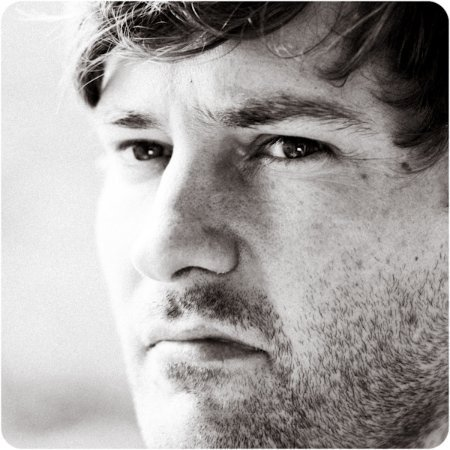
\includegraphics[width=0.6\columnwidth]{../media/borgsmidt.jpg}
	\vspace{-7cm}
\end{figure}

\begin{flushright}\footnotesize
  +45 71 77 03 23\\
  \href{mailto:rasmus@borgsmidt.dk}{rasmus@borgsmidt.dk}\\
  \href{http://dk.linkedin.com/in/borgsmidt}{linkedin.com/in/borgsmidt}\\
  \href{https://github.com/borgsmidt}{github.com/borgsmidt}\\[12pt]
  {\em Referencer udleveres\\ efter ønske}
\end{flushright}\normalsize
\framebreak

\fontdimen2\font=1.25\fontdimen2\font% interword space
\fontdimen3\font=1.25\fontdimen3\font% interword stretch
\fontdimen4\font=\fontdimen4\font% interword shrink

% Right frame
%%%%%%%%%%%%%%%%%%%%
\huge{\textbf{Rasmus Borgsmidt}} \\
\Large{\color{SpotColor}\em Erfaren software-udvikler,$\;$ bachelor i datalogi fra DIKU}

\normalsize\normalfont

\Sep\begin{inlinepar}{kort om mig}
  Født 1975 og opvokset i Københavnsområdet\Dot Leget med computere siden
  1980\-erne\Dot Bachelor i datalogi fra DIKU\Dot Ansat hos Adaytum i 1997, så
  opkøbt af \mbox{Cognos} i 2003 og IBM i 2009\Dot 15+ års erfaring i udvikling
  af software til finansiel planlægning\Dot Har arbejdet på talrige projekter
  med tekno\-logier rangerende fra ren maskinkode til OOP,
  funktionsprogrammering og array-sprog\Dot Opfinder og medopfinder på flere
  udstedte patenter\Dot Har boet fem år i England og Luxembourg\Dot Gift, far
  til tre, bor i København
\end{inlinepar}

\Sep\CVSection{erfaring}

\CVItem{Ledende software-udvikler,$\;$ IBM,$\;$ 2009--2014}

I denne rolle var min primære opgave at videreudvikle og vedligeholde den
centrale beregningskomponent i software-produktet {\em IBM Cognos Planning}. Jeg
deltog også i udviklingen af andre relaterede produkter og var ind imellem ude
hos kunder under beta-test af nye versioner af produktet.

\SmallSep\CVItem{Scrum master for et hold af udviklere,$\;$ IBM,$\;$ 2009--2012}

Ud over mine udviklingsopgaver havde jeg også en overgang rollen som {\em scrum
  master/holdkaptajn} for et hold af udviklere spredt over fire tidszoner.

\SmallSep\CVItem{Ledende software-udvikler,$\;$ Cognos,$\;$ 2003--2008}

I denne rolle var min primære opgave at udvikle og vedligeholde centrale
server\-komponenter i software-produktet {\em IBM Cognos Planning}. Derudover
var jeg ofte involveret i forskningsprojekter, som senere resulterede i en række
patenter.

\SmallSep\CVItem{QA-tekniker / software-udvikler,$\;$ Adaytum,$\;$ 1997--2002}

I min første rolle hos Adaytum arbejdede jeg med kvalitetssikring og med
udvikling af testsystemer. Senere fik jeg andre ansvarsområder og begyndte at
bidrage direkte til udviklingen af software-produktet {\em Adaytum Planning}.

\Sep\CVSection{uddannelse}

\CVItem{Bachelor i datalogi,$\;$ Københavns Universitet (DIKU),$\;$ 2010--2014}

Et bachelorprojekt blev afleveret juni 2013 og blev bedømt til karakteren
12. Afhandlingen (på engelsk) med titlen {\em Functional Array Programming
  Compiled to a Virtual Machine} udleveres efter ønske.

\SmallSep\CVItem{Bachelor i datalogi og matematik,$\;$ Københavns Universitet
  (DIKU),$\;$ 1994--1998}

Første forsøg på denne uddannelse blev afbrudt, kort efter jeg blevet ansat i
Adaytum.

\Sep\CVSection{færdigheder}

\begin{inlinepar}{programmering}
  Erfaring med en lang række sprog som f.eks.~Java, Ruby, C\#, JavaScript,
  Haskell, SML, Erlang, C, Python, J/APL, MSIL, Java Bytecode, assembler,
  maskinkode---og listen fortsætter.
\end{inlinepar}

\SmallSep\begin{inlinepar}{metode}
  Stærk tilhænger af {\em udefra-ind} designprincipper, som f.eks.~{\em
    test-driven development}, og forstår vigtigheden af små hold, gradvis
  levering af ny funktionalitet, samt iterative processer generelt. Anerkender
  det gode håndværk inden for software-udvikling og gør en dyd af kontinuert
  integrering og kodeforbedring.
\end{inlinepar}\enlargethispage{2\baselineskip}\\

{\hfill\footnotesize\em fortsætter på næste side}
\clearpage
\framebreak
\framebreak

\begin{inlinepar}{sprog}
  Taler og skriver flydende dansk og engelsk, samt tysk på almindeligt
  gymnasieniveau.
\end{inlinepar}

\Sep\CVSection{personlighed}
\begin{inlinepar}{træk}
  Altid nysgerrig, generelt vellidt, kan føre en meningsfuld samtale med alle
  slags mennesker. Håndterer pres godt og nyder at gøre ting på den rigtige
  måde.
\end{inlinepar}

\SmallSep\begin{minipage}{0.7\textwidth}
\begin{multicols}{3}
\begin{compactitem}[\hspace{12pt}\color{SpotColor}\NoSpaceDot]
	\item {\em holdspiller}
        \item {\em grundig}
        \item {\em kreativ}
        \item {\em analytisk}
        \item {\em går forrest}
        \item {\em professionel}
\end{compactitem}
\end{multicols}
\end{minipage}\\

\SmallSep\begin{inlinepar}{interesser}
  {\em Concurrent} programmering (Erlang/OTP)\Dot Dynamiske sprog og
  funktionssprog\Dot Grammatikker og DSLer\Dot Cloud\Dot Raspberry
  Pi\Dot Netværks\-sikkerhed og anonymitet\Dot Fotografi\Dot Emulering af
  klassiske computere\Dot Go (gammelt strategisk brætspil)
\end{inlinepar}

\Sep\CVSectionEm{patenter}{på engelsk}

\CVItem{Scalable mechanism for resolving cell-level access from sets of
  dimensional access rules},$\;$ 2013,$\;$ uspatno.~8,538,990\\[3pt]
Techniques for resolving cell-level access in a multi-dimensional data structure
based on one or more sets of dimensional access rules.\\[3pt]
Rasmus Borgsmidt, David Bowen, Kirk Bates

\MedSep\CVItem{Automatically moving annotations associated with
  multi-dimensional data be-\linebreak tween live data cubes},$\;$ 2013,$\;$
uspatno.~8,347,207\\[3pt]
Techniques for sharing multi-dimensional data and associated annotations between
software systems.\\[3pt]
Rasmus Borgsmidt, Finuala Barnes, Bindhu Cherian

\MedSep\CVItem{Enterprise planning and performance management system
  providing type-safe retrieval of multi-dimensional data},$\;$ 2011,$\;$
uspatno.~7,895,150\\[3pt]
Techniques for ensuring type safety at compile time of multi-dimensional data
retrieval.\\[3pt]
Rasmus Borgsmidt, Michael Gould

\MedSep\CVItem{Job scheduling for automatic movement of
  multi-dimensional data between live data cubes},$\;$ 2011,$\;$
uspatno.~7,877,355\\[3pt]
Techniques for sharing multi-dimensional data between software systems.\\[3pt]
Rasmus Borgsmidt, David Bowen

\MedSep\CVItem{Virtual multi-dimensional datasets for enterprise
  software systems},$\;$ 2010,\\
uspatno.~7,747,562\\[3pt]
Techniques for specifying virtual datasets within an enterprise
software system.\\[3pt]
Rasmus Borgsmidt, Michael Gould

\MedSep\CVItem{Multi-dimensional data cube validation},$\;$ 2009,$\;$
uspatno.~7,610,294\\[3pt]
Techniques for validating data that a user enters into a multi-dimensional data
cube within an enterprise software system.\\[3pt]
Rasmus Borgsmidt
\end{document}
